%%%%%%%%%%%%%%%%%%%%%%%%%%%%%%%%%%%%%%%%%%%%%%%%%%%%%
%				  Video In module					%
%					-----------						%
% Author: Vaibhav Singh	& Thibault Porteboeuf 		%
%%%%%%%%%%%%%%%%%%%%%%%%%%%%%%%%%%%%%%%%%%%%%%%%%%%%%

\section{Video-In module}
\begin{figure}[H]
\center
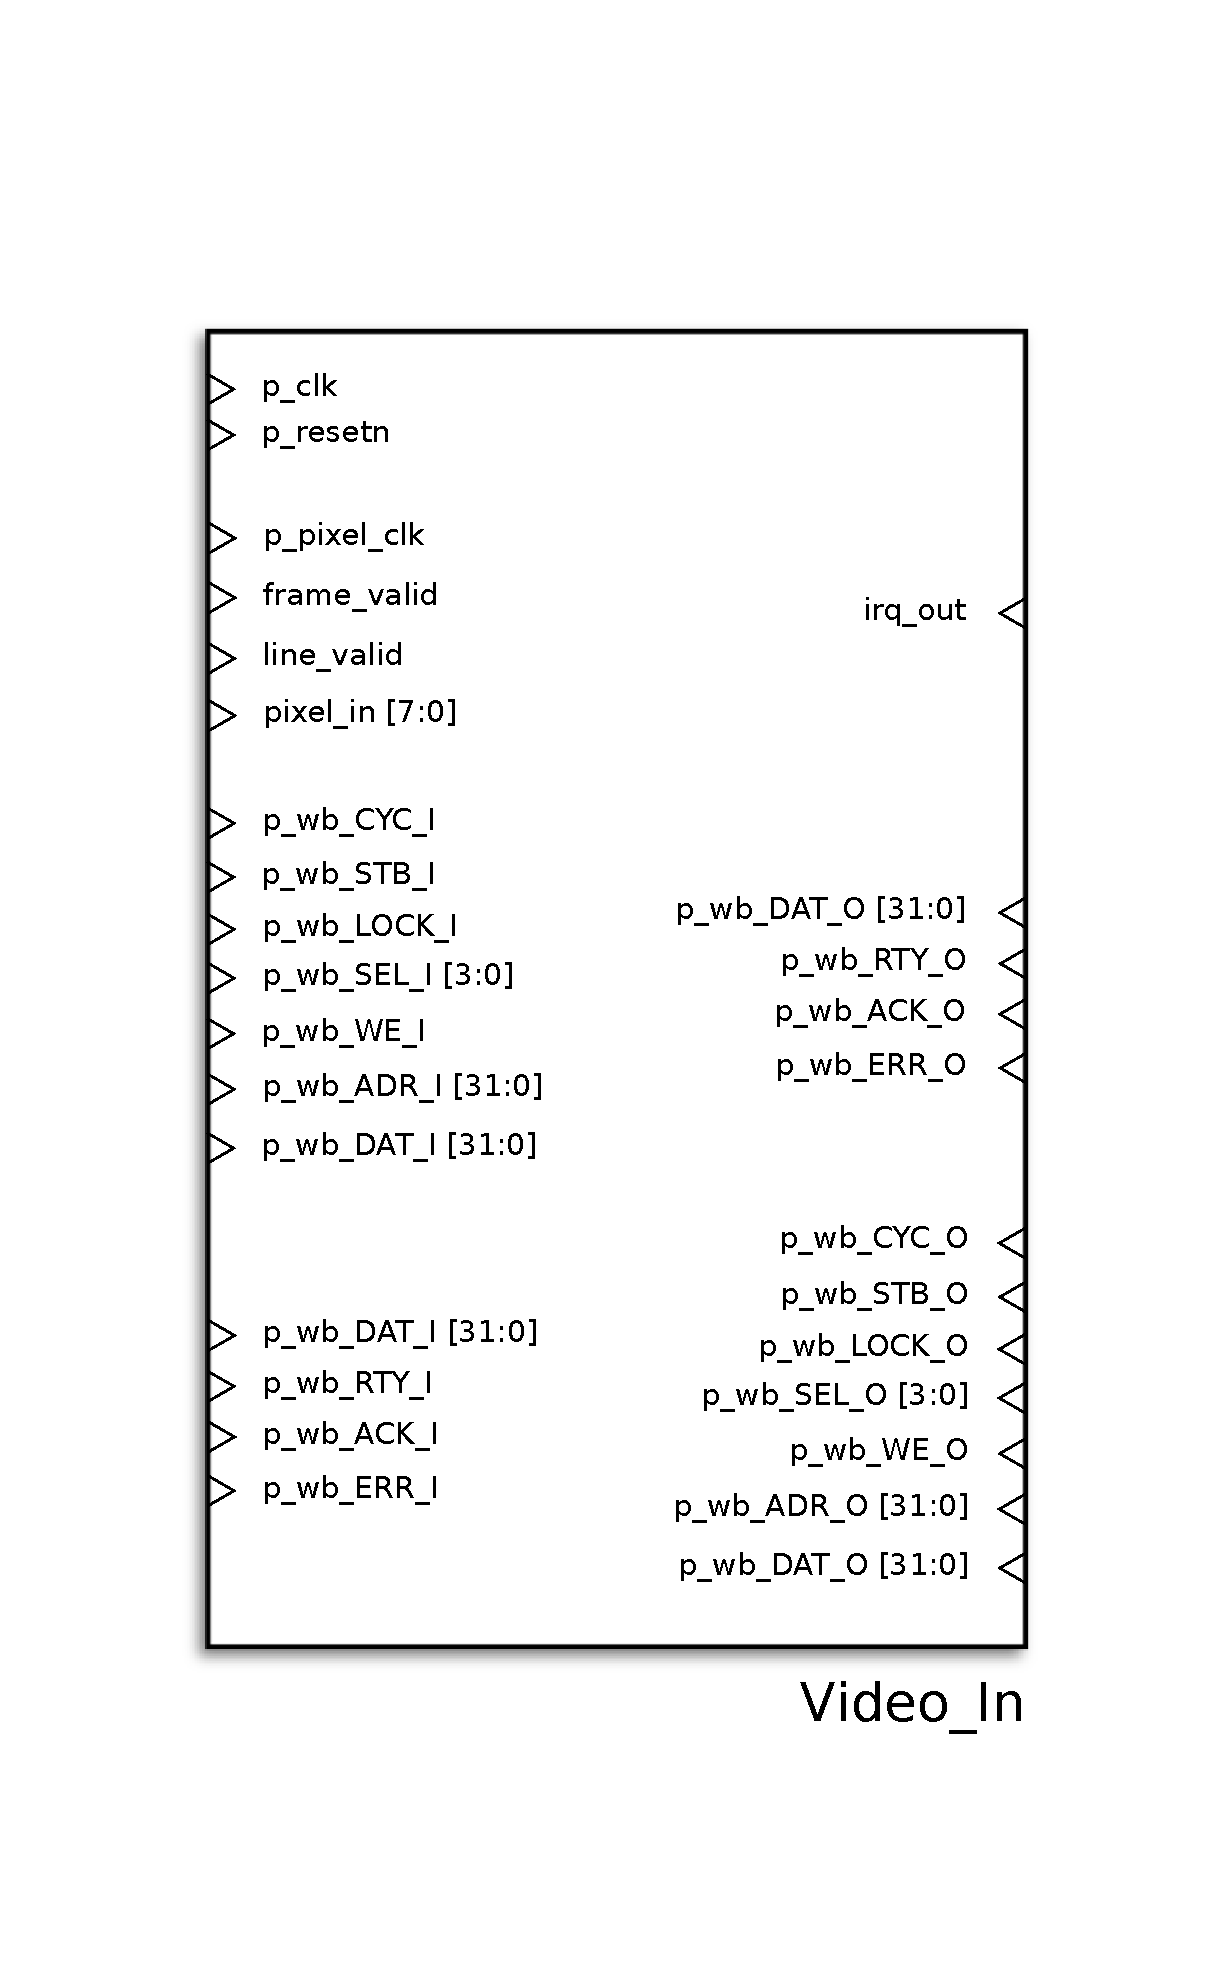
\includegraphics[width=7cm]{figs/Video_in.pdf}
\caption{Video-In module's interface}
\label{VideoIn_interface}
\end{figure}

As explained before, Video-In is the module responsible for handling the incoming video signals and transfer the pixels to the RAM over the whishbone bus.

As described in the figure below, Video In Module has a Wishbone Master Module and a one register slave, as described in section \ref{wb_reg_slave}.

Video In has two blocks, one that takes pixels from video generator running at a frequency of 25 Mhz, and an other one that stores data on to RAM. Synchronisation of internal signals between the two different clock domains has been done by sampling the 25 Mhz clock, using the system's 100 Mhz clock.

The wishbone slave will handle incoming requests from the LM32, and store the content of write requests (start address of images) to its register. It is also responsible for driving the Irq (Interrupt Request) wire which will be raised to high whenever video in requests a new start address from the LM32. The slave will automatically acknowledge when a write request is received.

The state machine samples the configuration stored in the slave's register at every rising edge of the \texttt{frame\_valid} signal. Thus, the configuration is updated only at the beginning of a new frame.

It then posts data from the buffer to the RAM, starting at the previously given address. This process is illustrated in figure \ref{VideoIn_sm}. 

It is important to notice that, following the idea that the peripherals are driven and configured by the LM32, the VideoIn module will remain Idle until the LM32 activates it by carrying a first write request to VideoIn's slave.

Detailed explanation of video in can be found along the explanation of the source code.

\begin{figure}[h]
\center
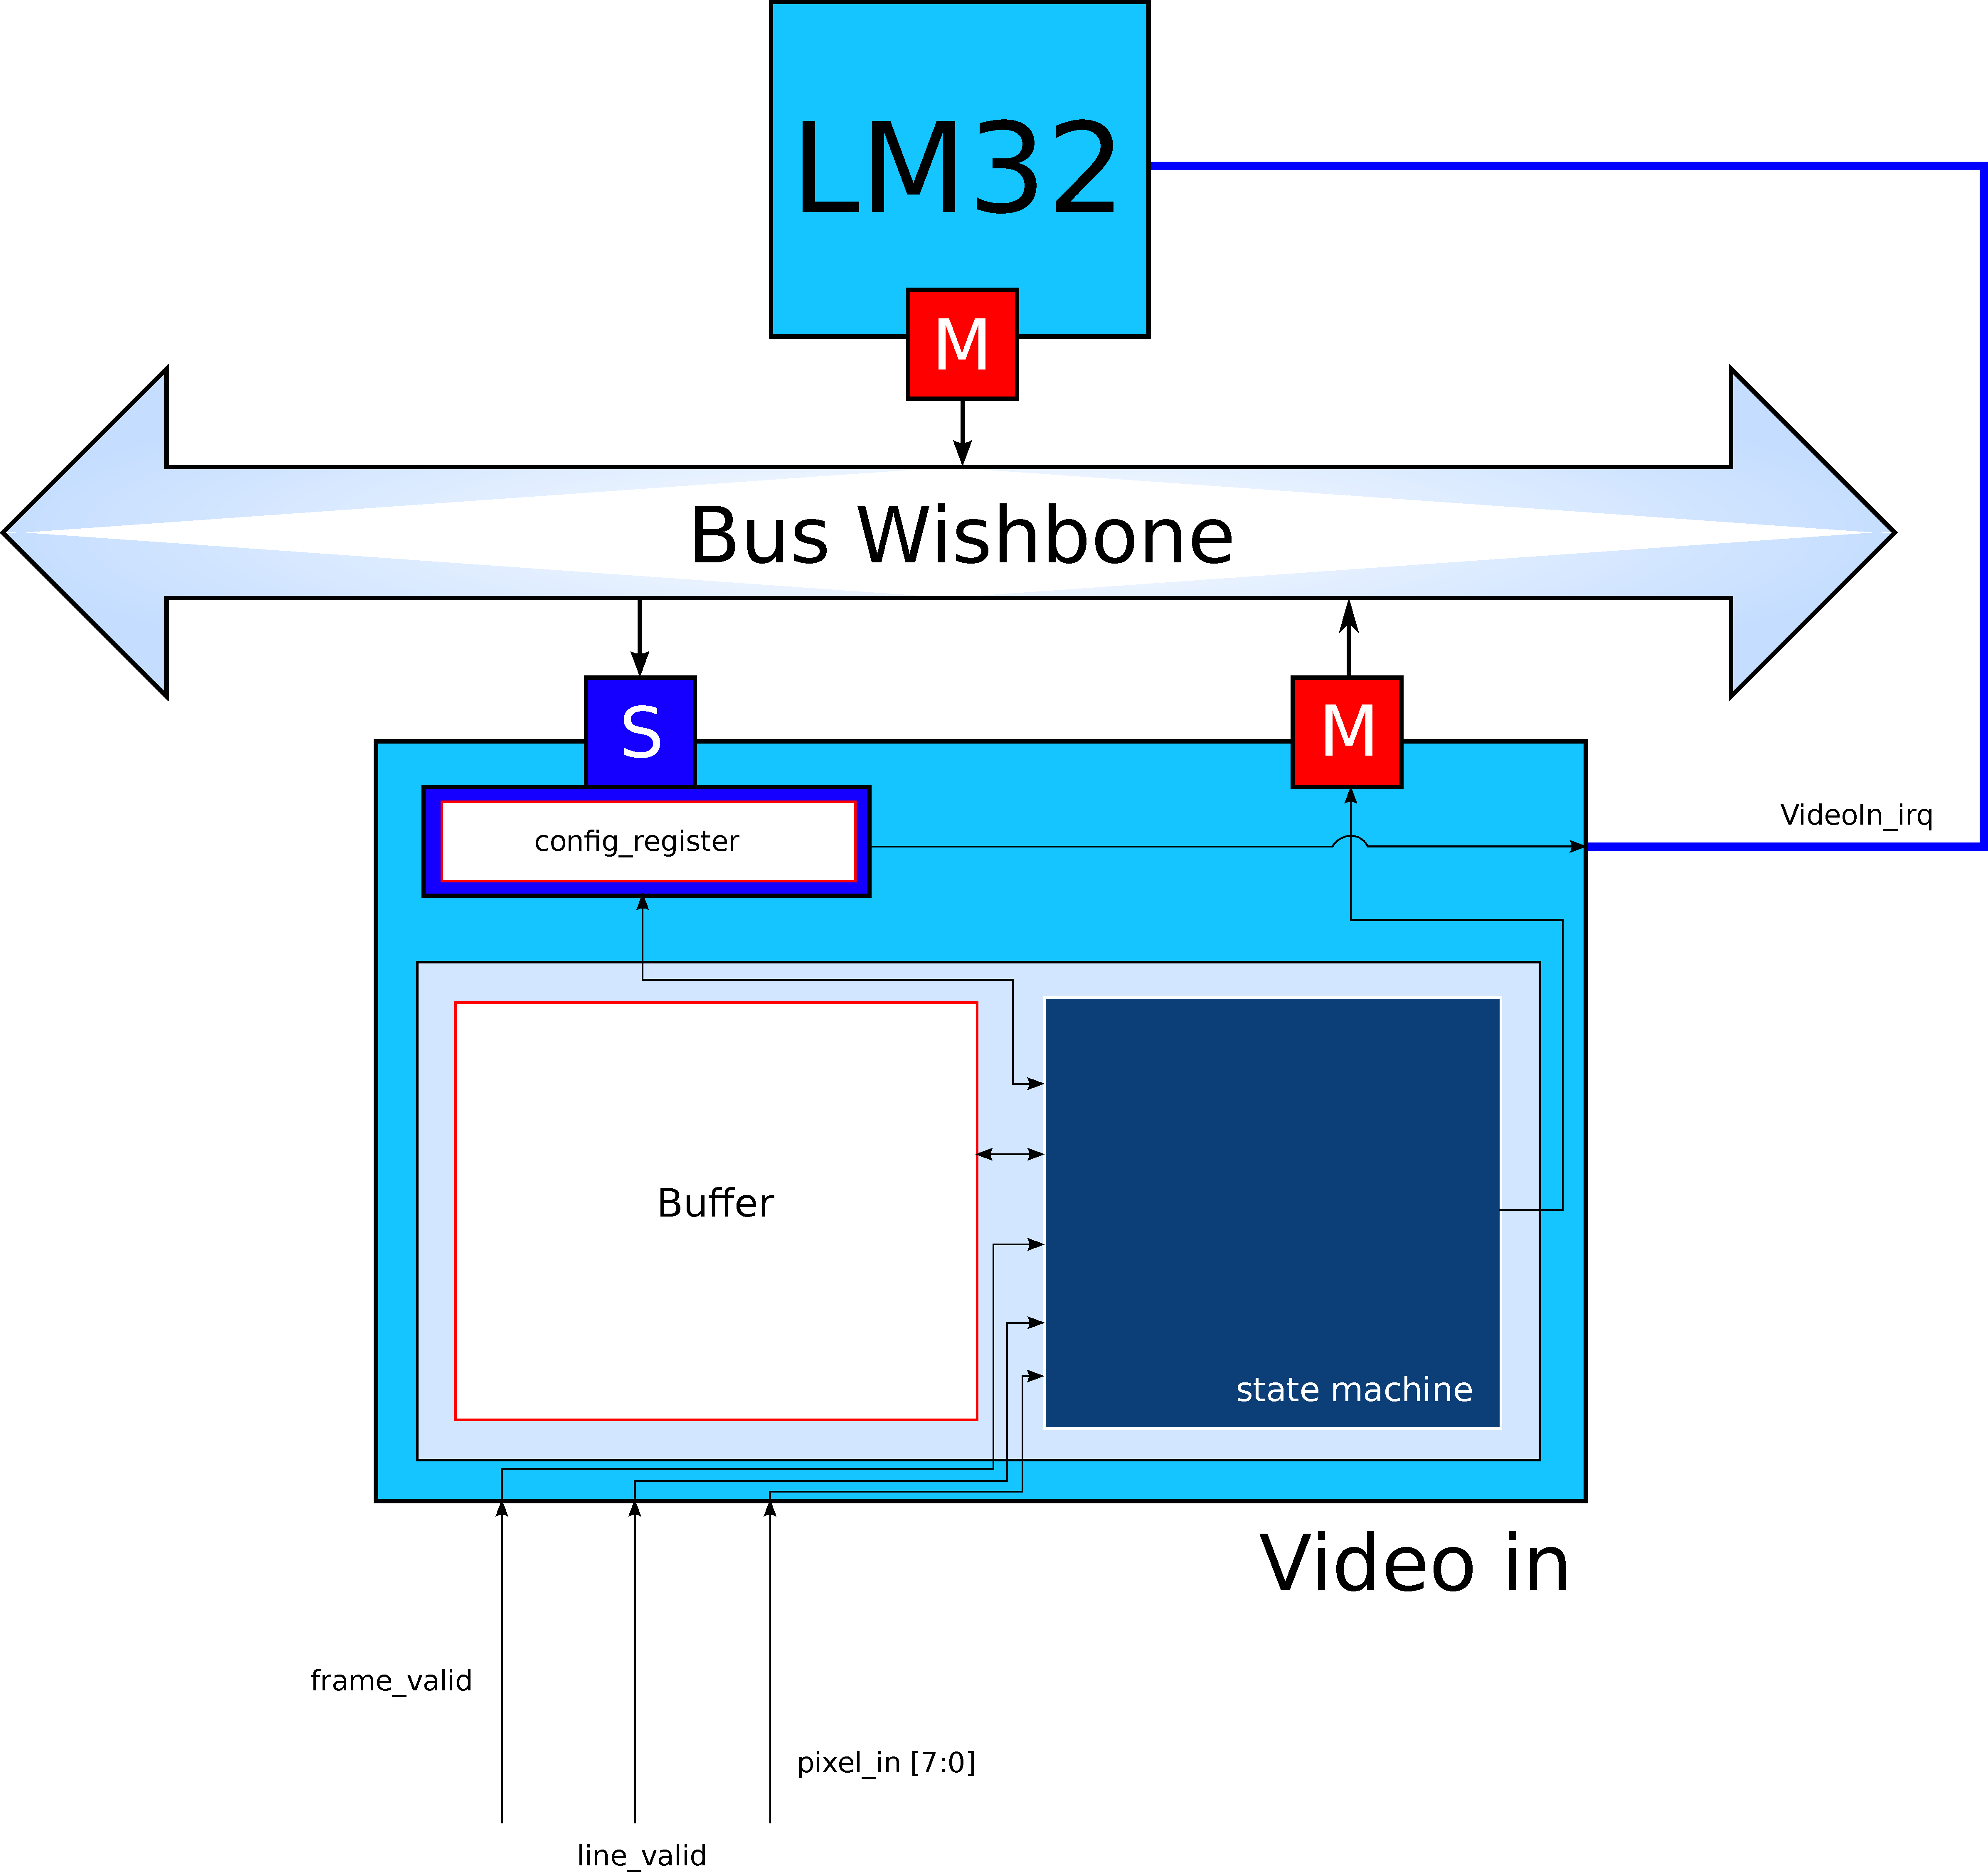
\includegraphics[width=11cm]{figs/Video_In_blocks.pdf}
\caption{VideoIn's inner structure}
\label{VideoIn_struct}
\end{figure}


\begin{figure}[h]
\center
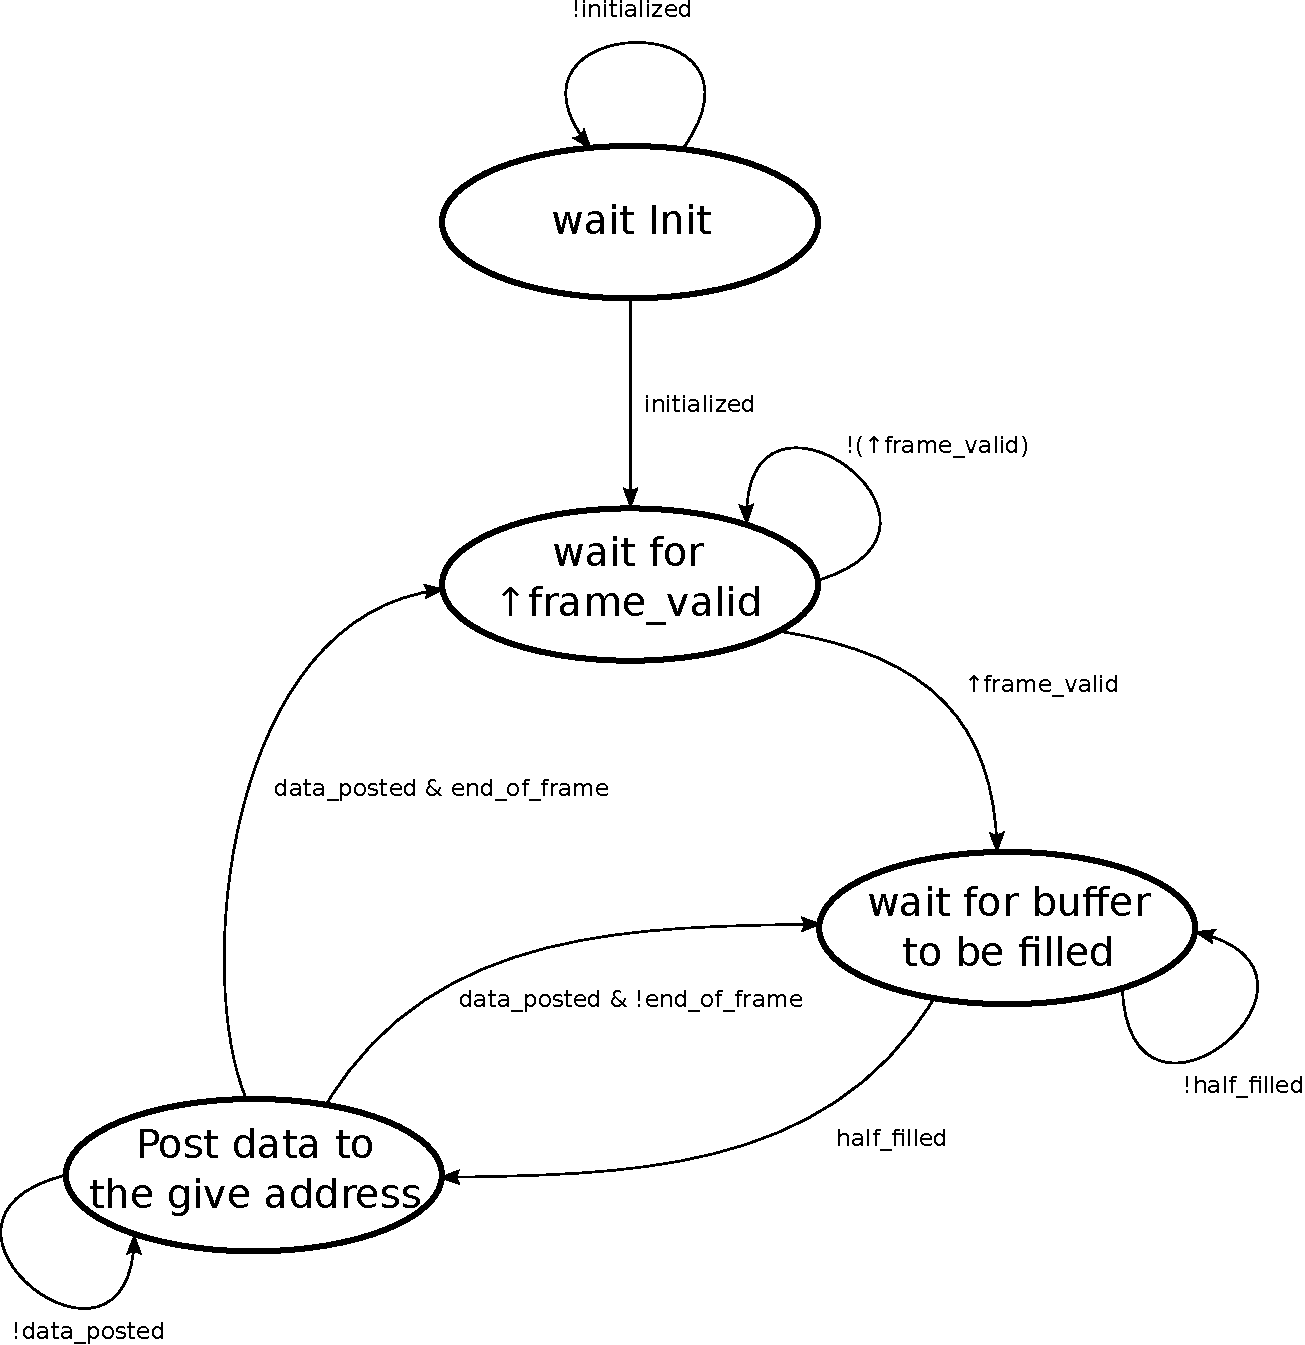
\includegraphics[width=11cm]{figs/video_in_sm.pdf}
\caption{VideoIn's behavior}
\label{VideoIn_sm}
\end{figure}

